\chapter{Introduction and Background}
%\textcolor{red}{chapter 1 is Ready to revised}\\
Over the last few decades wireless networks have been established as one of the promising technology to provide communication with the ease of mobility and data reliability. The ever increasing demand for data rate and connectivity anywhere, anytime are the main motivations \textcolor{black}{for an intensive use of multi-antenna communication systems.} By deploying Multiple-Input Multiple-Output (MIMO) system, where multiple antennas are installed at both transmitter and receiver, it is possible to increase the capacity and efficiency \textcolor{black}{of wireless networks with respect to more conventional Single-Input Single-output (SISO) based systems}. MIMO systems are one of the keystones in the development and extension of data-intensive applications like  and social  media and video streaming on hand held devices, surveillance and navigation systems for target detection and tracking, also health based applications using intra-body communications (IBC).\\
However, this improvement in performance gain and reliability also \textcolor{black}{increases processing and hardware costs and creates new challenges. Therefore, the requirement to develop efficient digital signal processing (DSP) based algorithms and multiple access techniques is indispensable to tackle this challenge.}
\section{Background}
The main challenges to enhance system performance in communication system \textcolor{black}{derive from \textit{fading} which is due to changes in transmission medium or paths which cause time variation of received signal power, and \textit{interference,} mainly caused by the fact that more than one user share the same radio resources at the same time.} In more details, transmitted signals can reach the receiver by more than one paths because of scatters and obstacles in the medium, this phenomena is called multipath \textcolor{black}{interference. %Undoubtedly, to improve the system performance either we should built some techniques to avoid interference or by making signals orthogonal within the given spectrum. Multipath propagation of radio signals from transmitter to receiver results in diverse spatial characteristics. 
MIMO systems may be designed to counteract this multipath radio arrangement, resulting in better performance and reliability.}
To increase system reliability and data rate in MIMO system, two types of data transmission arrangement are generally used. In \textit{transmit/receive diversity} identical data is transmitted/received by multiple antennas, \textcolor{black}{improving signal reliability, while keeping the same system throughput. Different types of MIMO architectures are shown in figure \ref{mimo}.
\begin{figure}
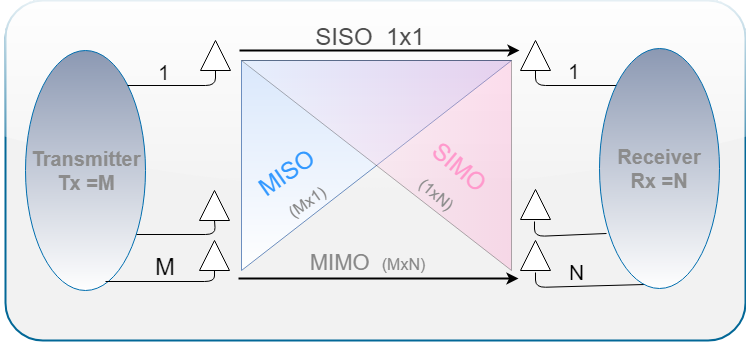
\includegraphics[scale=0.8]{figures/MIMO.png}
\caption{Diversities in Multi-terminal system}
\centering
\label{mimo}
\end{figure}
On the other hand, if independent data streams are transmitted from each antenna, MIMO systems could effectively increase the system throughput. In this case, the scheme is called space division multiple access (SDMA) or multi-user MIMO (MU-MIMO).}
%The MIMO systems are developed by considering existing spectrum resources, 

%\textcolor{black}{COMMENT: I think the following remaining part of this chaper needs to be modified. I think that these details on MIMO must be insterted in a more specific chapter (for instance the next chaper on wireless comms). I think you need to generally introduce the other topics of the thesis, like CS, channel recovery, intrabodyc comms, by trying to consider all of them under the main topic of MIMO communications}
Since spectrum is a limited and expensive resource it must be utilized efficiently. \textit{Spectral efficiency} determine the rate of information transmitted per unit bandwidth. Another important metric to keep in mind other than spectral efficiency  while measuring performance in wireless system is \textit{energy efficiency (EE)}. Energy efficiency can be achieved by optimizing the transmit power.
To mitigate interference across multiple users in MU-MIMO different types of \textit{beamforming or precoding} techniques can used at transmitter: 
\begin{itemize}
    \item \textbf{Analog Beamforming:} In analog beamforming, analog phase shifters are used to steer the beam in the direction of the user \cite{bjornson_book}. Multiple beams can be formed to serve different users, but it depends on number of antennas and size of array used \cite{thesis_xiang}. To serve different users simultaneously, the possible beams that can be formed must be orthogonal to each other, a limiting factor to analogue beamforming.
    \item \textbf{Digital beamforming/Precoding:} The digital beamforming or linear precoding, is performed in baseband \textcolor{black}{ where the different user signals are }superimposed with varying power and phase. Digital beamforming is more flexible and simple \textcolor{black}{than} analog beamforming, and its complexity does not grow with the number of antennas.
\end{itemize}

\section{Compressed Sensing}
\textcolor{black}{Due to multiple nodes, MIMO systems are computationally expensive and their energy requirement is also high. The main reason \textcolor{black}{is the }high level of signal processing techniques \textcolor{black}{needed }to mitigate interference among nodes as they are sharing channel resources. \textcolor{black}{Moreover,} the transmitter and receiver design become complicated to manage multi-antenna transmission. \textcolor{black}{These issues} can be handled, if we will be able to reduce the \textcolor{black}{signal }measurements with the help of some signal processing techniques. Compressive sensing (CS)  techniques \textcolor{black}{allow to } recover \textcolor{black}{a} signal with a much lower number of linear measurements than in the conventional case. \textcolor{black}{If respecting} the constraint that the underlying signal is sparse. \textcolor{black}{In this way},  the system can be made energy-efficient \textcolor{black}{by exploring the} underlying signal. Numerous examples can be given for signals which are sparse in some \textcolor{black}{particular domain like} time, frequency \textcolor{black}{and wavelet ones.} In the following, two real-world sparse signal cases are explained \textcolor{black}{in order to solve} some MIMO based problems \textcolor{black}{discussed in this thesis}.
\begin{itemize}
    \item \textcolor{black}{In} massive MIMO \textcolor{black}{system }most of the channel energy lies only on few dominant taps \cite{sparse_channel}, therefore its channel impulse response (CIR) will be sparse. This is due to the large number of antennas at the base station (BS) with only few scatters at the BS side (compared to the number of antennas), hence only  few active transmission directions per user, hence the channel matrix tends to be sparse \cite{mainref-joint,exp-vitual}.
\item \textcolor{black}{For} humans in intra-body communications (IBC) system efficiency is directly related to the energy \textcolor{black}{consumption} and security related issues.
In practical applications, implants may not transmit data
continuously. Hence, we can easily assume that the sensed data is sparse, and with the help of the CS framework sufficient energy efficiency can be achieved, without degrading the performance.
\end{itemize}
\section{\textcolor{black}{MIMO Applications} }
In this thesis three \textcolor{black}{MIMO} applications have been considered and their \textcolor{black}{related} research problems have been solved with the help of signal processing techniques.
 \subsection{Massive MIMO}
 Massive MIMO or large scale MIMO is a natural extension of conventional MIMO, \textcolor{black}{and} it groups large number of antennas at \textcolor{black}{the }BS to improve spectral efficiency and throughput in mobile communication. By employing large number of antennas at BS,  the system capacity is increased tremendously, because of spatial multiplexing techniques \textcolor{black}{and }higher data rates can be achieved. Beamforming techniques help massive MIMO \textcolor{black}{systems} in getting better area coverage by \textcolor{black}{optimizing the} received signal power. Moreover, it reduce the latency by using parallel detection\cite{latency} and by combating fading dips with the help of optimal beamforming \cite{magazine_eric}.
 Due \textcolor{black}{to} immense benefits of MIMO systems, \textcolor{black}{they have} become essential  part of many latest standards \textcolor{black}{such as} WLAN (802.11n, 802.11ac etc.), WiMAX (IEEE 802.16e), LTE, LTE-Advanced, etc.
 \subsection{MIMO in Intra-Body Communication}
  Intra-body communication (IBC), is a data communication technique in which human body is used as a \textcolor{black}{transmission medium} or channel. Multiple implants are embedded into the human body \textcolor{black}{in order to} sense and forward their data to \textcolor{black}{a} skin node, called relay. These implants are interconnected and work in a MIMO fashion that allows internal physiological data to be gathered in real time and analyzed offline, thereby, transforming personalized medicine.
   The theoretical background can be developed for
   beamforming using an array of implants acting as distributed MIMO antennas. Significant performance gain can be achieved with the help of beamforming techniques in IBC. However, there are several challenges associated with IBC \textcolor{black}{, like} for example, energy efficiency, interference among implants, synchronization issues, etc.  
 \subsection{Cross-polarization interference canceller (XPIC)} 
   In the evolution of fifth-generation (5G) \textcolor{black}{mobile} communication technologies, there is always an increasing demand for user traffic, resulting in higher bandwidth requirement.
Cross polarization interference cancellation (XPIC) technology
represents the enabler for dual-polarized transmissions over the
same radio frequency (RF) channel, so that the link capacity is
doubled by using two orthogonal polarization channels over the
same link. In cross-polar transmission \textcolor{black}{the} 
same carrier frequency is utilised for simultaneous
transmission/reception of two different data streams.
Basically, \textcolor{black}{one} antenna is sending information on the same carrier, \textcolor{black}{by exploiting different horizontal and vertical} polarizations. The \textcolor{black}{considered} XPIC transmission is based on two independent and unsynchronized transceiver paths for backhaul links, with completely independent transmitter and receiver local oscillators (LOs).   }
 
%The key advantages in general MIMO based system compared to SISO based system are:
%\begin{itemize}
%    \item Increase capacity, because of spatial multiplexing techniques in MIMO higher data rates can be achieved.
   % \item Reliability, in MIMO system with the help of diversity and better digital signal processing algorithm data reliability is improved.
 %   \item Better area coverage is achieved by deploying BF(beamforming), which provide optimal received signal power.
 %   \item Reduced fading effects by employing different diversity techniques in frequency, time and space.
%    \item Reduced latency by using parallel detection  \cite{latency} and by combating fading dips with the help of optimal beamforming \cite{magazine_eric}.
%\end{itemize}
%Because of immense benefits MIMO system it has already been standardized in latest wireless standards namely, WLAN (802.11n, 802.11ac etc.), WiMAX (IEEE 802.16e), LTE, LTE-Advanced etc.
%MIMO system benefits can be extended by employing more antennas at the transmitter, a natural extension of MIMO system, massive MIMO.
\section{Problem Description and Main Contribution}
This research is devoted to the analysis of MIMO based system challenges and to the development of robust algorithms and techniques to handle them. We have considered different types of MIMO system research problems.
\begin{enumerate}
\item \textbf{Channel Estimation:}
Firstly, to overcome the limitation of traditional \textcolor{black}{architecture}, large scale MIMO or massive MIMO has been proposed in \cite{mimo_eric1,mimo_eric2}. Massive MIMO not only improves the spectral and energy efficiency but also helps to mitigate inter-user interference \cite{mimo-gain}. Although, massive MIMO  solves many traditional MIMO problems, but it opens completely new research avenues. 
In more detail, with a large number of transmit antennas at BS in massive MIMO, the degree of freedom is also increased, making the system more reliable and robust with reduced error rate and high throughput. With promising throughput, it is also expected that massive MIMO can serve many users simultaneously. However, supporting multiple users simultaneously is challenging due to inter-user interference, that can be mitigated if each user has its aligned beam, which can be attained with beamforming/precoding \footnote{by beamforming we are always referring digital beamforming}. 
Uplink (UL) combining or downlink (DL) transmit beamforming require good channel state information (CSI) \textcolor{black}{ that} can be attained using time division duplex (TDD) or frequency division duplex (FDD). \textcolor{black}{In TDD scheme channel reciprocity can be used to estimate downlink channel via uplink training. However, in TDD with large number of transmit antennas, base station is assumed to serve more users simultaneously which produces severe problem of pilot contamination because of the utilization of non-orthogonal pilots \cite{mimo_eric2}. Although FDD do not enjoy this channel reciprocity, as UL and DL are in separate band but it is generally considered more robust to delay-sensitive applications \cite{FDD_or_TDD}. Moreover, most of the existing systems are \textcolor{black}{employing} FDD, therefore it is of great importance \textcolor{black}{investigating } different approaches to obtain CSI in FDD.}\\
     In FDD massive MIMO channel estimation, the main problem is the pilot training and feedback overhead which increases with the number of transmit antennas, compromising the advantages of massive MIMO \cite{Dict_learning}.
     Therefore, pilot training \textcolor{black}{and feedback overhead} reduction techniques have been presented and \textcolor{black}{compared} with the existing research works. The results show that \textcolor{black}{the proposed} system outperform existing schemes.
    % Moreover, in addition to pilot overhead reduction technique algorithmped for limited feedback in a partially joint channel.The comparison has been carried out with state of the art algorithms, and results shows that our presented system is more efficient than previously proposed one. 
 \item \textbf{Synchronization:} We have considered the issues related to synchronization in MIMO based systems \textcolor{black}{developing such techniques for } cross-polarization interference cancelling (XPIC) system. Reduced complexity Kalman based algorithms are proposed to recover the phase of XPIC receiver in microwave radio relay links.
 %For the fulfillment of high data rate demand, accurate and realizable synchronization and beamforming techniques are indispensable.  With the help of such synchronization techniques,  MIMO system can achieve a higher link capacity by using higher-order modulation schemes(i-e QAM)\cite{our_kalman}. For that reason, we have considered XPIC, or
 \textcolor{black}{\item \textbf{Beamforming Galvanic Coupling Signals:}\\
 The state of the art for Intra-Body Communication (IBC) relies on high frequency radio (RF) signals. RF based systems are not energy efficient \textcolor{black}{from the point of view of } IBC. Additionally, emitted RF signals may extend to several feet around the body, creating privacy risks. We employed an alternative wireless architecture for IBNs using galvanic coupling (GC), in which low or medium frequency ($100\,\mathrm{kHz}$-$1\,\mathrm{MHz}$) and weak ($\leq 1\,\mathrm{mW}$) electrical currents are modulated with data and directly coupled to the tissue. The privacy risks related to RF are eliminated by using GC in IBNs since the signals do not propagate outside the skin layer \cite{teshome}. In GC based system currents are used in place of classical radio frequency (RF) links.\\
 As the first step, we devise a
method that allows multiple implants to communicate individual
sensed data to each other through code division multiple access (CDMA) combined with compressive sensing (CS) method to
lower the transmission time and save energy, as well as delegates
the computational burden of despreading and decoding only
to the on-body surface relays. Then, we devise a distributed
beamforming approach that allows coordinated transmissions
from the implants to the relays by considering the specific tissue
path chosen and tissue heating-related safety constraints.We then
proceed to implement distributed beamforming on a phantom of
human tissue and prove an increase in received signal strength
and decrease in BER due to constructive interference of the
signals of each implant.}
\end{enumerate}

\section{Thesis Organization}
%\textcolor{black}{COMMENT: please replace "we have" with a more formal in third person, in all the following sentences}
%\textcolor{olive}{ done}\\
{The Chapter 2}, presents MIMO system in general and the theoretical underpinnings of MU-MIMO. Also, the assumptions and challenges while dealing with channel estimation in  MIMO are discussed.\\
%ofdm, types of beamforing, equalization
{The Chapter 3}, presents a brief introduction to the essentials of compressive sensing theory in context of sparse channel estimation and most widely used sparse signal recovery algorithms.\\
%signal recovery, sensing matrix,algorithm classification 1)greedy algorithms and convex optimizatio based,
{The chapter 4}, covers the pilot reduction techniques for sparse channel estimation in massive MIMO systems. We exploit compressive sensing (CS) techniques to accurately estimate the channel, while assuring overhead reduction which is proportional to the sparsity level of the channel. 

{The Chapter 5}, have discussed joint Sparse Channel Recovery with Quantized feedback for Multi-User Massive MIMO Systems. In this chapter, a distributed compressed sensing based novel algorithm, 2-step quantized partially joint orthogonal matching pursuit (Q-PJOMP) is proposed which not only reduce training overhead but also recover the channel from limited feedback for FDD based multi-user massive MIMO.

{In chapter 6}, a novel method is  devised that allows multiple implants in intra-body network to communicate individual sensed data to each other through code division multiple access (CDMA) combined with compressive sensing (CS) method to lower the transmission time and save energy and lower computational burden.

{In chapter 7}, the research work is presented on galvanic coupling (GC) technology.A sound card based GC testbed is designed and implemented to achieve  high flexibility and real time physiological data sets transmissions.

{Chapter 8}, discussed the reduced complexity Kalman filtering for phase recovery in XPIC systems. In this work, two completely independent radio frequency (RF) transceiver chains are considered for the two different polarization's, in order to have the maximum flexibility to connect different single carrier transceivers to dual-polarized antennas.\\

%\textbf{In chapter 10}, the issue of multipath interference in multi-receiver FMCW RADAR is investigated for multi-layer snow-pack.





%beamforming helps us to take the advatge of spatial muliplexing(pararel channels in space) without interferece.


%TDD and FDD difference  Realizing massive MIMO with Time Division Duplexing (TDD) operation is convenient, due to the inherent Uplink-Downlink (UL-DL) channel reciprocity [2]. In contrast, channel reciprocity does not hold in Frequency Division Duplexing (FDD) operation, since UL and DL take places in different bands, which are separated by much more than the fading coherence bandwidth. Therefore, the UL channel state information (CSI) can not be used for DL data transmission, so that the BS has to probe the DL channel via training and ask for CSI feedback from the users\cite{FDDvsTDD}.










